\documentclass[11pt,a4paper]{article}

% Packages
\usepackage[utf8]{inputenc}
\usepackage[T1]{fontenc}
\usepackage{geometry}
\geometry{margin=2.5cm}
\usepackage{graphicx}
\usepackage{booktabs}
\usepackage{hyperref}
\usepackage{amsmath}
\usepackage{caption}
\usepackage{subcaption}
\usepackage{float}
\usepackage{enumitem}
\usepackage{xcolor}
\usepackage{listings}

\hypersetup{
    colorlinks=true,
    linkcolor=blue,
    urlcolor=blue,
    citecolor=blue
}

\lstset{
    basicstyle=\ttfamily\small,
    breaklines=true,
    frame=single,
    backgroundcolor=\color{gray!10}
}

\title{\textbf{HW2: Detect AI Generated Text}\\[0.3em]
\large RNN and Transformer — Comprehensive Report}
\author{Student}
\date{April 2026}

\begin{document}

\maketitle

\begin{abstract}
This report presents a comprehensive study on detecting AI-generated text using BERT-based classifiers. We fine-tune both \texttt{bert-base-cased} (108M parameters) and \texttt{bert-large-cased} (334M parameters) on the DAIGT V2 Train Dataset (44,868 essays), achieving ROC-AUC of 0.9999 for both models. We compare these against TF-IDF baselines (best AUC: 0.9997 with Linear SVM), conduct ablation studies on sequence length (512 vs 256 tokens) and training epochs (3 vs 5), and perform adversarial attacks using a locally deployed DeepSeek-R1:8B model via Ollama. The BERT detector proves highly robust: only 3/30 single-pass attacks (10\%) and 0/5 iterative attacks succeed. All experiments were conducted on an NVIDIA RTX 4090 GPU with fp16 mixed precision.
\end{abstract}

\tableofcontents
\newpage

% ============================================================
\section{Data Analysis \& Baseline (Part 1)}
% ============================================================

\subsection{Exploratory Data Analysis}

We analyzed four text-level features comparing human-written (Label 0) and AI-generated (Label 1) essays. Statistical significance was evaluated using the Mann-Whitney U test, with effect sizes measured by Cohen's $d$.

\begin{table}[H]
\centering
\caption{EDA: Feature comparison between human and AI text}
\label{tab:eda}
\begin{tabular}{lcccc}
\toprule
\textbf{Feature} & \textbf{Human (mean)} & \textbf{AI (mean)} & \textbf{Cohen's $d$} & \textbf{$p$-value} \\
\midrule
Avg Word Length     & 4.82  & 5.06  & $-0.733$ & $\approx 0$ \\
Word Count          & 271.3 & 280.5 & $+0.594$ & $\approx 0$ \\
Sentence Count      & 11.4  & 13.2  & $+0.384$ & $\approx 0$ \\
Type-Token Ratio    & 0.807 & 0.841 & $-0.366$ & $\approx 0$ \\
\bottomrule
\end{tabular}
\end{table}

All four features show statistically significant differences ($p \approx 0$). The strongest signal is \textbf{average word length} (Cohen's $d = -0.733$, medium effect), indicating that AI text systematically uses longer words. Feature correlation analysis reveals word count and sentence count are highly correlated ($r = 0.80$), while TTR is negatively correlated with word count ($r = -0.59$).

\begin{figure}[H]
\centering
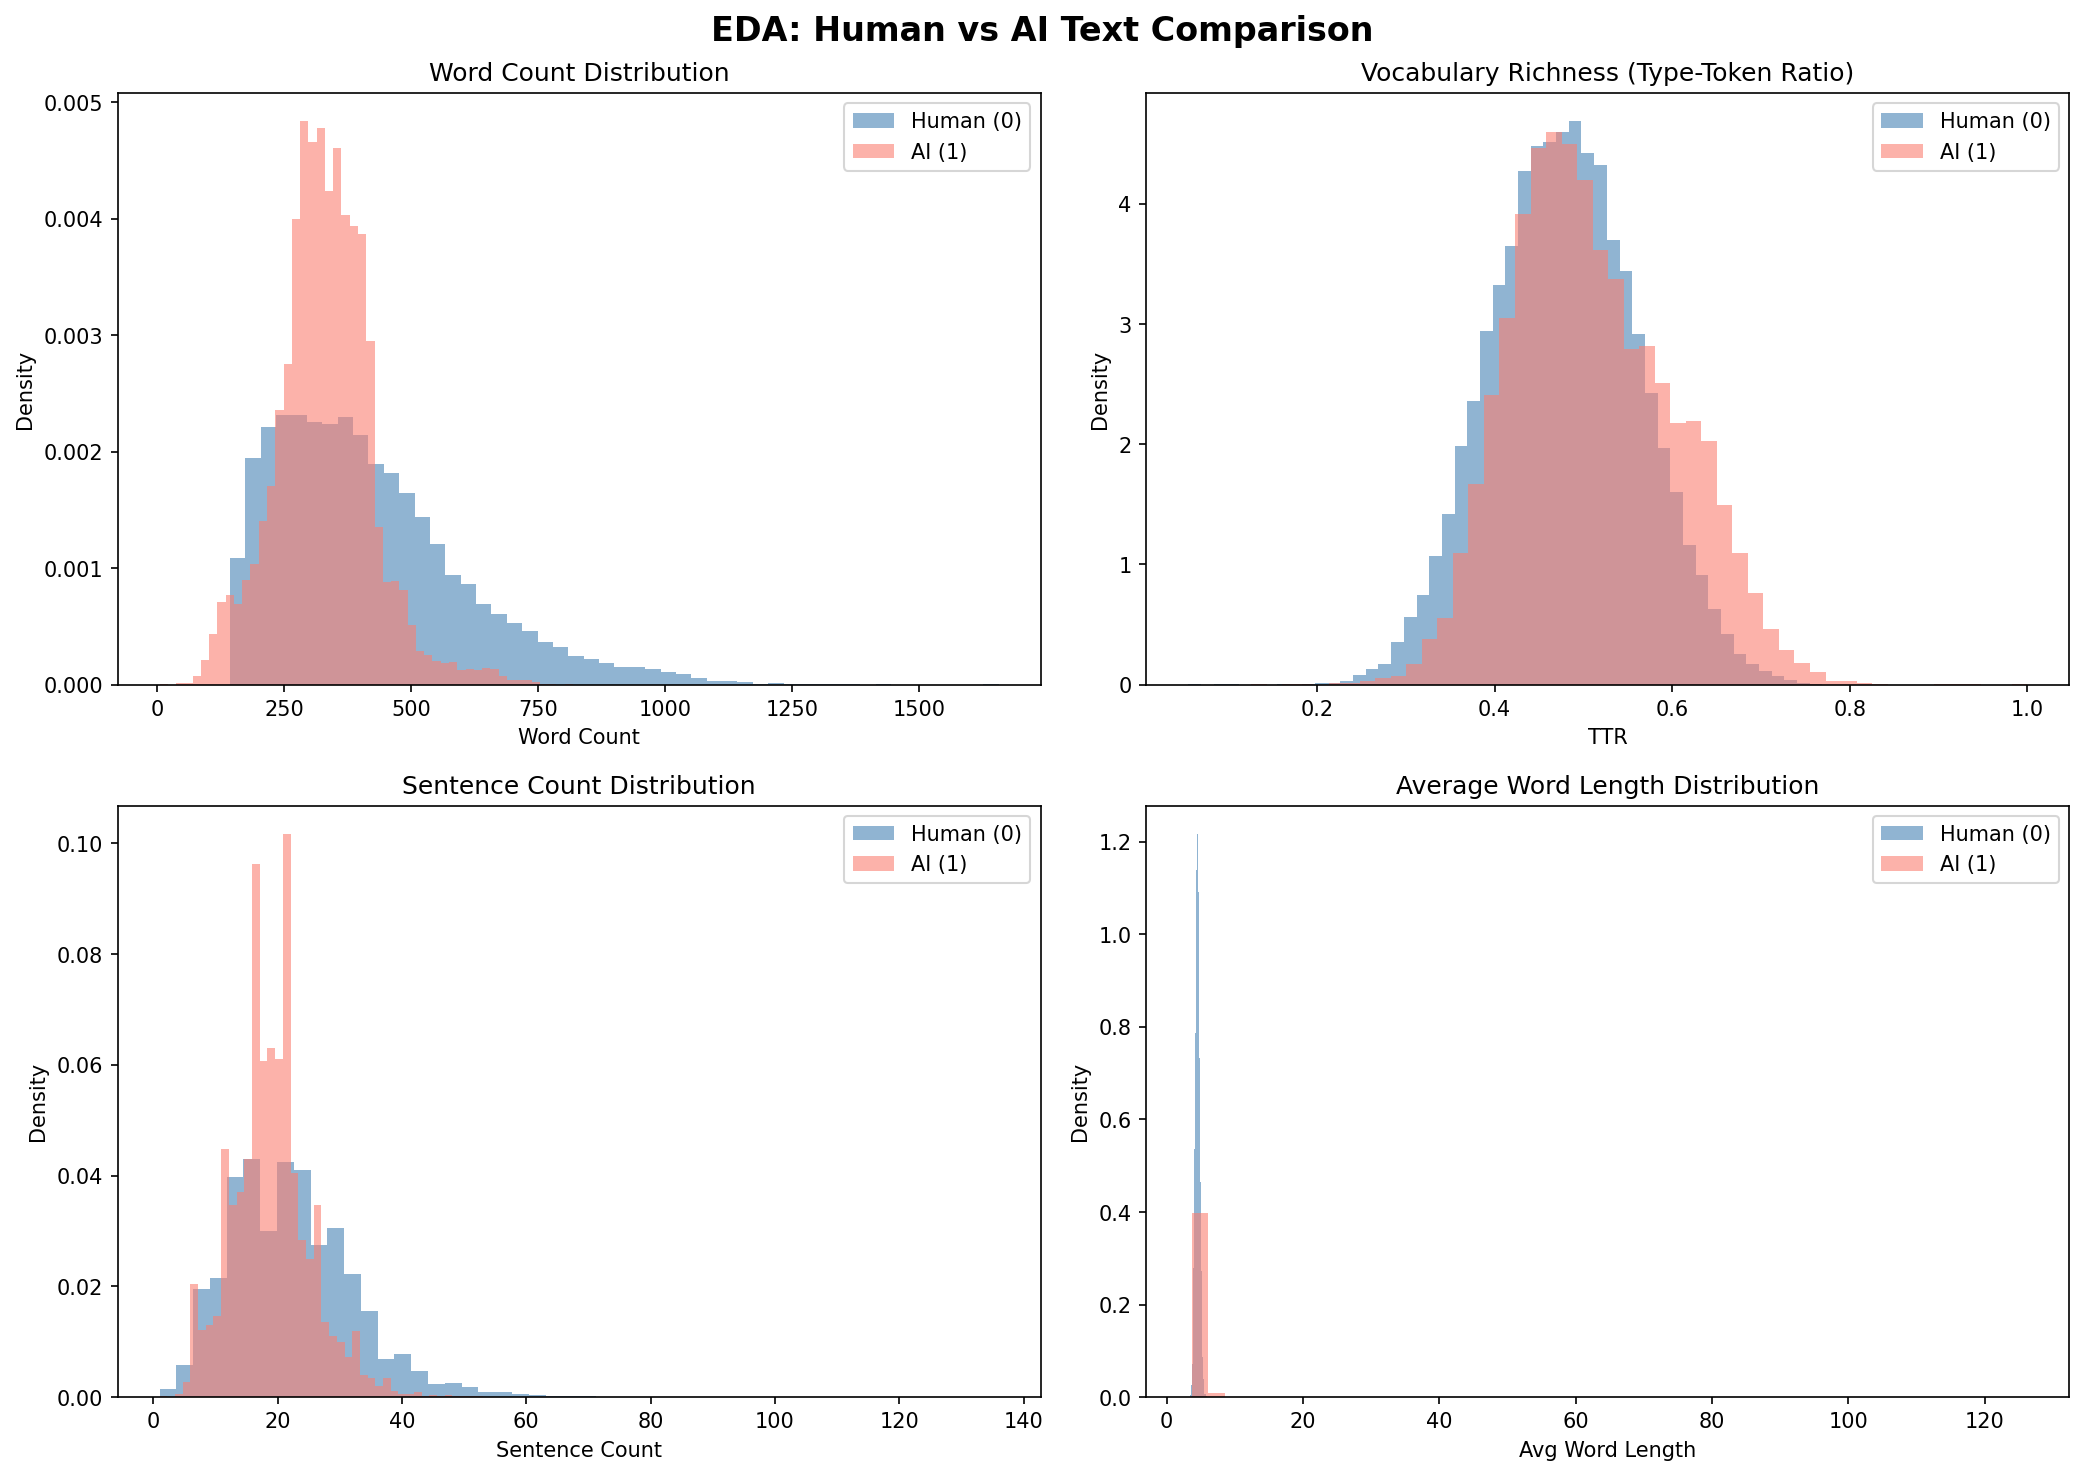
\includegraphics[width=0.85\textwidth]{results_baseline/eda_distributions.png}
\caption{Distribution comparison of text features between human and AI essays.}
\label{fig:eda}
\end{figure}

\begin{figure}[H]
\centering
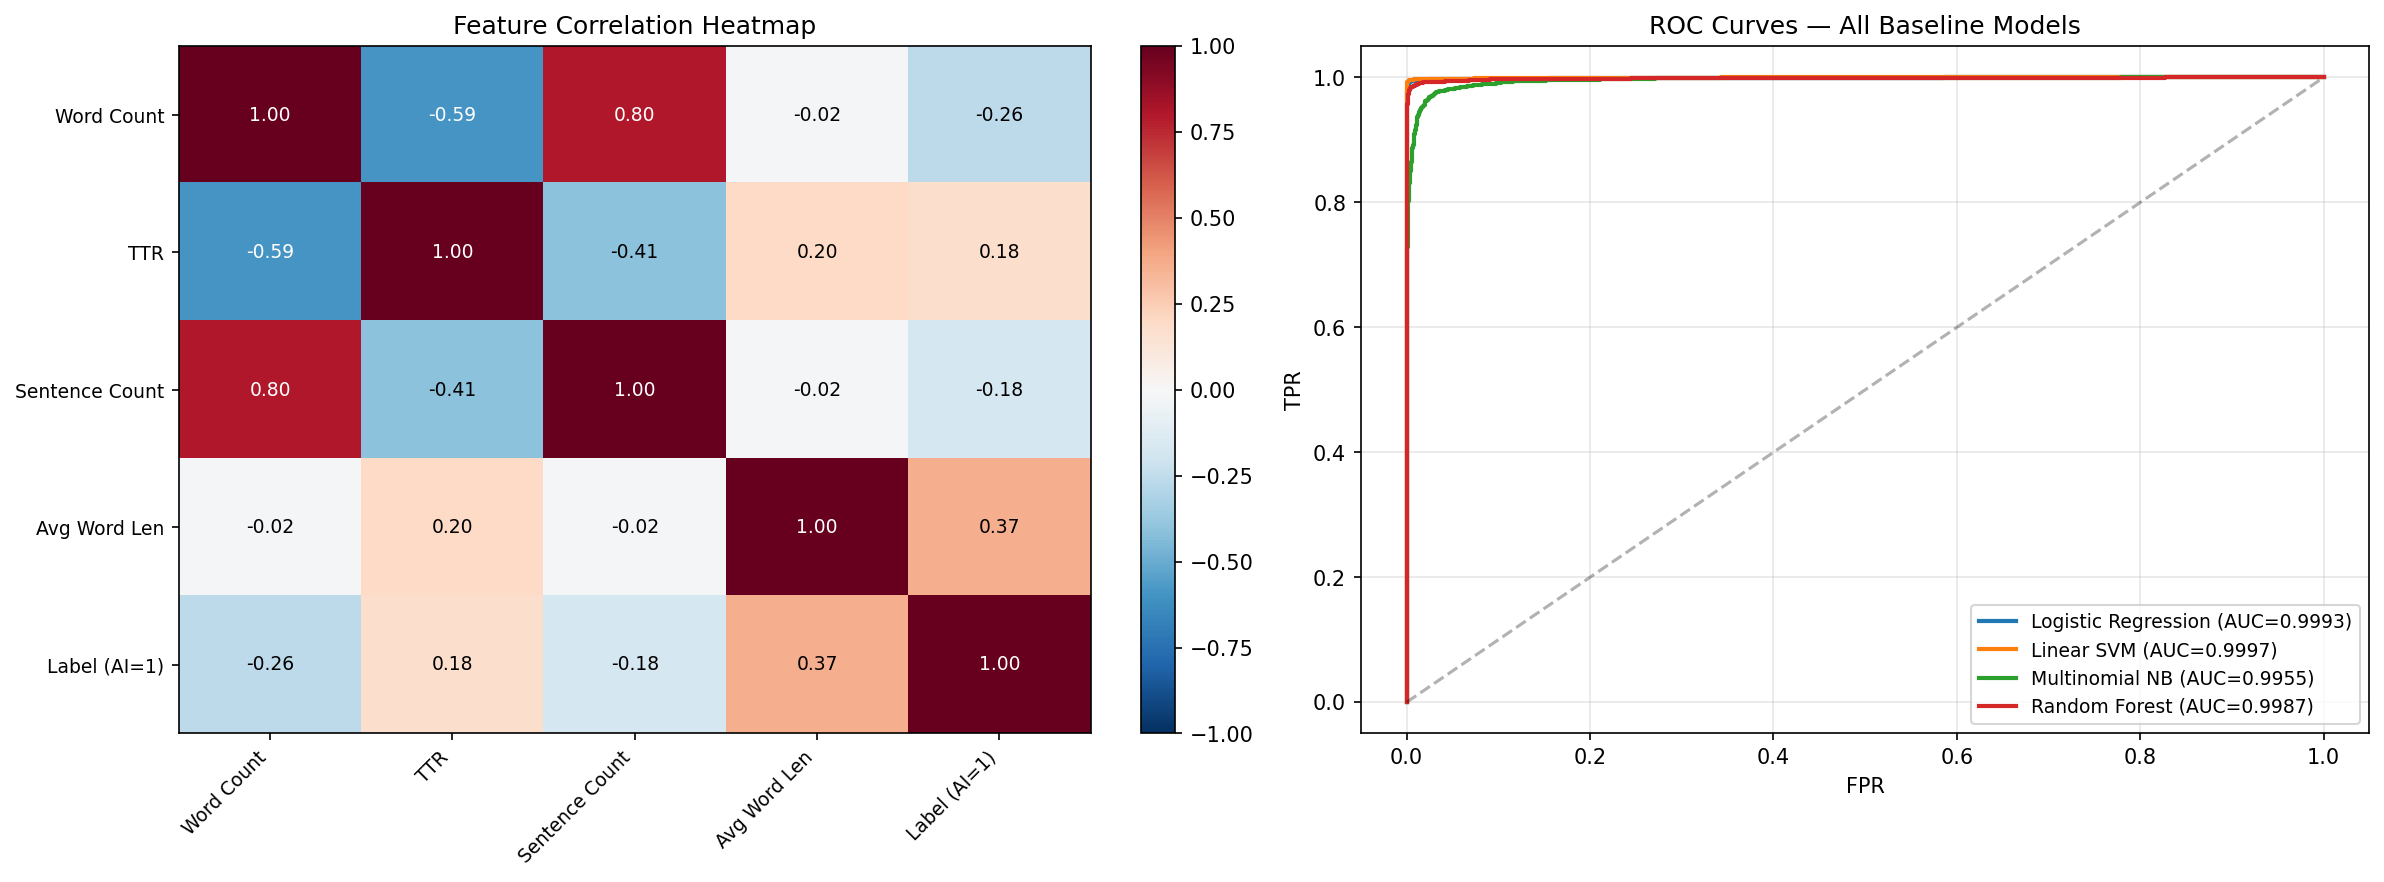
\includegraphics[width=0.85\textwidth]{results_baseline/enhanced_eda.png}
\caption{Feature correlation heatmap and all-baselines ROC comparison.}
\label{fig:enhanced_eda}
\end{figure}

\subsection{Baseline Models}

We implemented four classifiers using TF-IDF vectorization (max\_features=10{,}000, ngram\_range=(1,2)):

\begin{table}[H]
\centering
\caption{Baseline model performance (TF-IDF features)}
\label{tab:baseline}
\begin{tabular}{lccccc}
\toprule
\textbf{Model} & \textbf{ROC-AUC} & \textbf{Accuracy} & \textbf{Precision} & \textbf{Recall} & \textbf{F1} \\
\midrule
Logistic Regression      & 0.9993 & 0.9939 & 0.9980 & 0.9863 & 0.9921 \\
\textbf{Linear SVM}      & \textbf{0.9997} & \textbf{0.9970} & 0.9971 & 0.9951 & 0.9961 \\
Multinomial Naive Bayes  & 0.9955 & 0.9692 & 0.9781 & 0.9423 & 0.9598 \\
Random Forest (200 trees)& 0.9987 & 0.9884 & 0.9968 & 0.9734 & 0.9850 \\
\bottomrule
\end{tabular}
\end{table}

Linear SVM achieves the highest baseline AUC (0.9997), approaching BERT-level performance. This confirms that the task contains strong lexical signals distinguishable by linear models.

\begin{figure}[H]
\centering
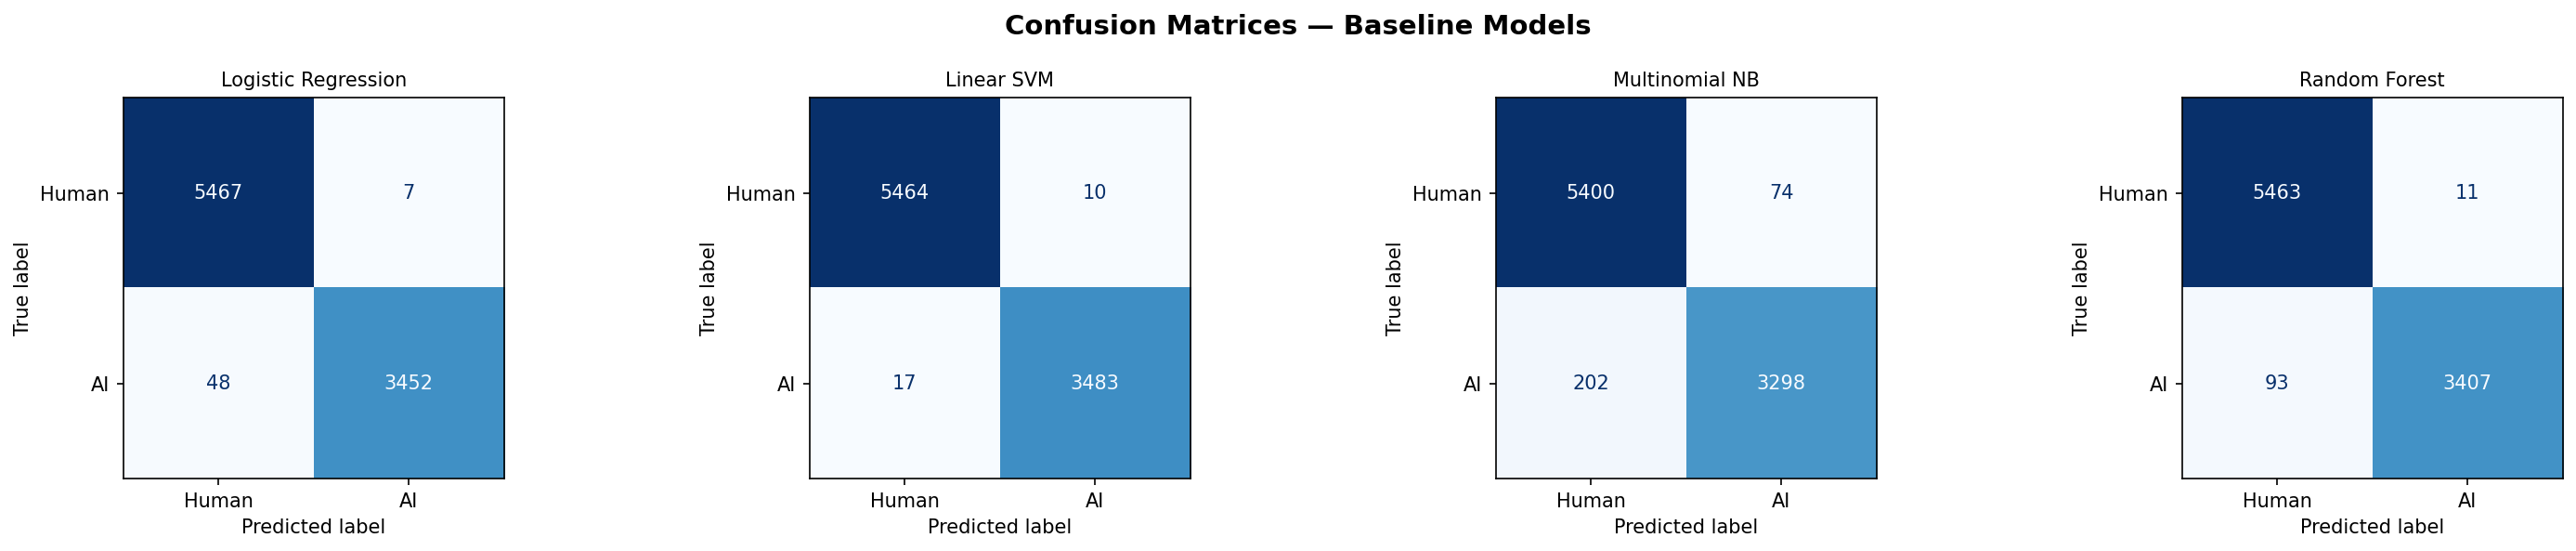
\includegraphics[width=0.85\textwidth]{results_baseline/baseline_confusion_matrices.png}
\caption{Confusion matrices for all four baseline classifiers.}
\label{fig:baseline_cm}
\end{figure}

% ============================================================
\section{BERT Fine-Tuning \& Scaling (Part 2)}
% ============================================================

\subsection{Experimental Setup}

\begin{itemize}[nosep]
\item \textbf{Models}: \texttt{bert-base-cased} (108M params), \texttt{bert-large-cased} (334M params)
\item \textbf{Tokenizer}: \texttt{AutoTokenizer.from\_pretrained()} with matching checkpoint
\item \textbf{Training}: HuggingFace \texttt{Trainer} API, fp16 mixed precision, AdamW optimizer
\item \textbf{Hyperparameters}: learning\_rate = $2 \times 10^{-5}$, weight\_decay = 0.01, warmup\_ratio = 0.1
\item \textbf{Data split}: 80/20 stratified train/validation
\item \textbf{Hardware}: NVIDIA RTX 4090 (24GB VRAM)
\end{itemize}

\subsection{Results}

\begin{table}[H]
\centering
\caption{BERT fine-tuning results across all experiments}
\label{tab:bert}
\begin{tabular}{lccccr}
\toprule
\textbf{Experiment} & \textbf{Params} & \textbf{ROC-AUC} & \textbf{Accuracy} & \textbf{Batch} & \textbf{Time} \\
\midrule
BERT-base (3ep, len=512)  & 108M & 0.9999 & 0.9941 & 32 & 8.3 min \\
BERT-base (3ep, len=256)  & 108M & 0.9997 & 0.9899 & 32 & 4.0 min \\
BERT-base (5ep, len=512)  & 108M & 0.9999 & 0.9967 & 32 & 14.3 min \\
BERT-large (3ep, len=512) & 334M & 0.9999 & 0.9974 & 16 & 26.1 min \\
\bottomrule
\end{tabular}
\end{table}

\begin{figure}[H]
\centering
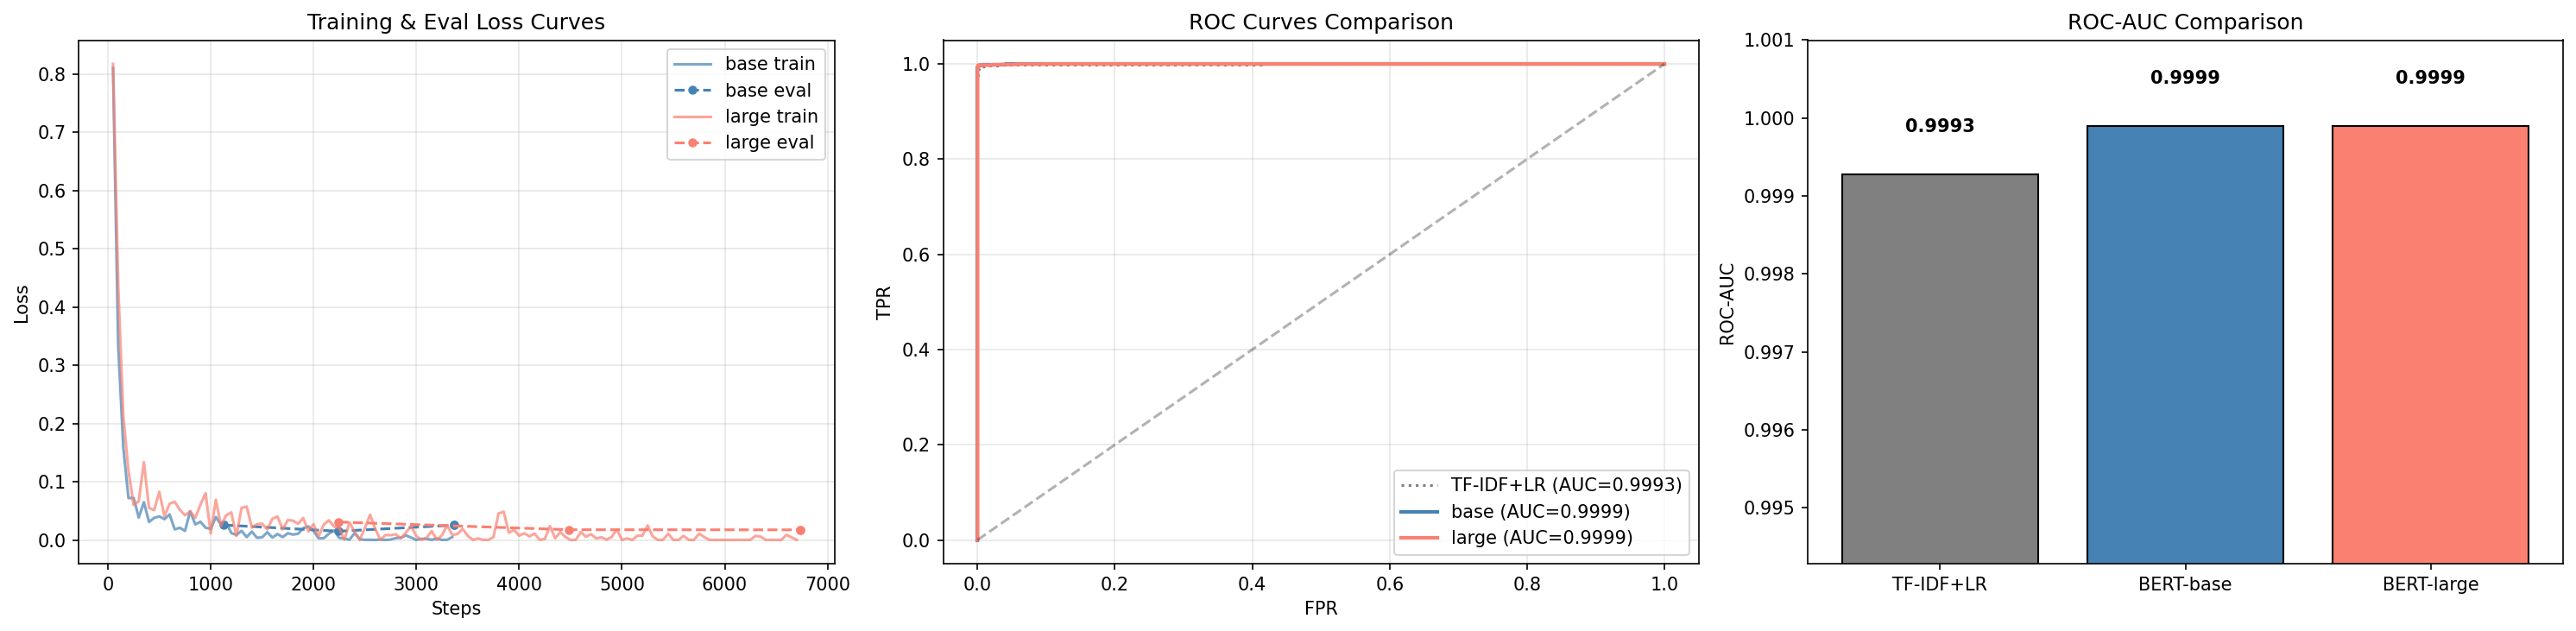
\includegraphics[width=0.95\textwidth]{results_bert-base-cased/comparison_curves.png}
\caption{Left: Training \& evaluation loss curves for BERT-base and BERT-large. Center: ROC curves comparison (TF-IDF vs BERT). Right: ROC-AUC bar chart.}
\label{fig:comparison}
\end{figure}

\subsection{Scaling Analysis}

\subsubsection{Model Size: Base vs Large}

Both BERT-base and BERT-large achieve \textbf{identical ROC-AUC (0.9999)}. BERT-large provides marginally higher accuracy (0.9974 vs 0.9941, +0.33 pp) and a lower false positive rate (0.26\% vs 0.86\%), but requires $3\times$ the parameters and $3.1\times$ the training time. The marginal gain does not justify the computational cost --- the task saturates at 108M parameters.

\subsubsection{Sequence Length: 512 vs 256}

Reducing max\_length from 512 to 256 causes only a \textbf{0.0002 AUC drop} ($0.9999 \to 0.9997$) while \textbf{halving training time} ($8.3 \to 4.0$ min). This suggests most classification signal is concentrated in the first 256 tokens. For deployment, 256-token models offer nearly identical performance at half the inference cost.

\subsubsection{Epoch Count: 3 vs 5}

Five epochs with BERT-base achieves Accuracy 0.9967 (vs 0.9941 at 3 epochs) with the same AUC 0.9999. Loss curves confirm the model converges by epoch 2--3; epochs 4--5 provide marginal accuracy gains without overfitting.

\begin{figure}[H]
\centering
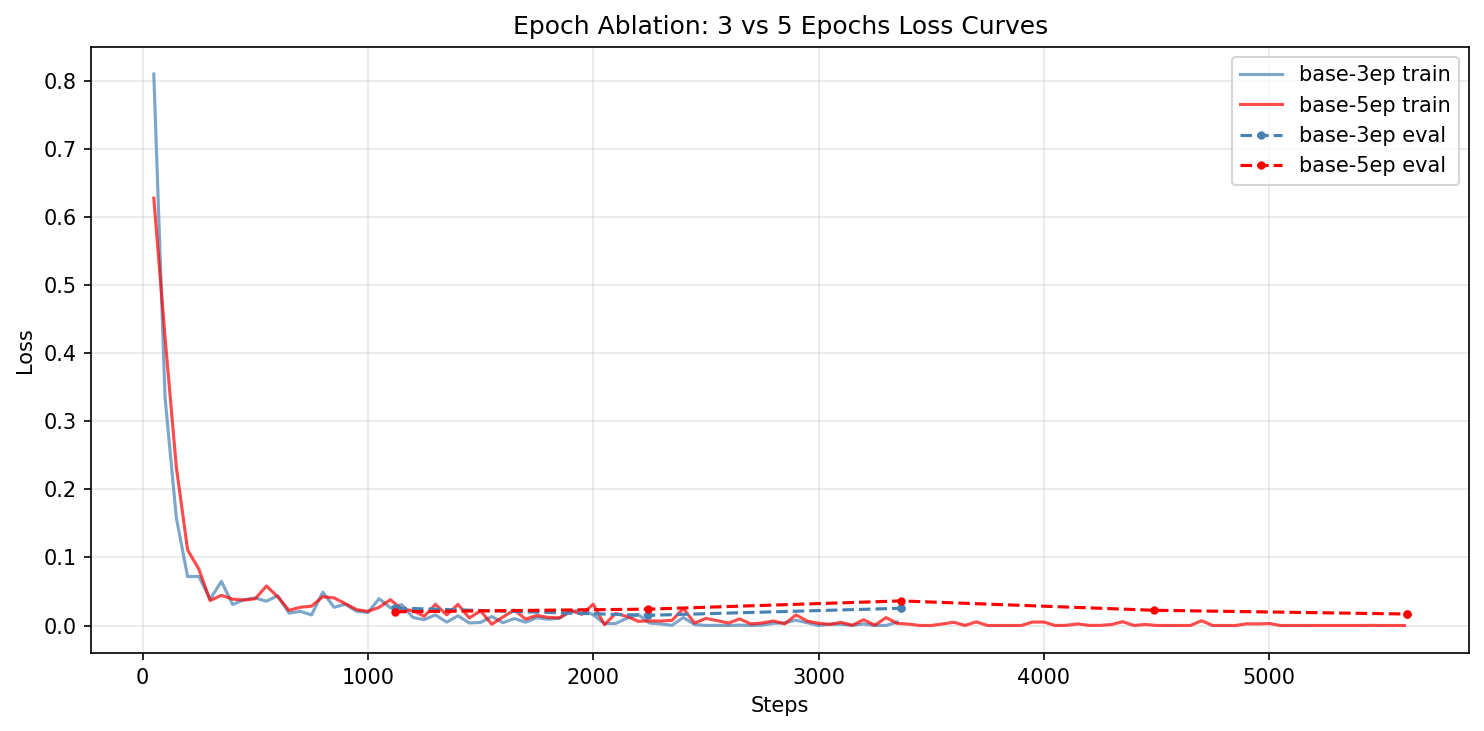
\includegraphics[width=0.7\textwidth]{results_bert-base-cased/epoch_ablation.png}
\caption{Epoch ablation: Training loss comparison between 3-epoch and 5-epoch BERT-base.}
\label{fig:epoch_ablation}
\end{figure}

\subsection{Hypothesis: Does Large Outperform Base?}

\textbf{No.} Both models achieve ROC-AUC = 0.9999 on this task. The task is ``saturated'' --- the discriminative signal between human and AI text is strong enough that even a 108M-parameter model captures it fully. The primary differences are in error profiles. This saturation is further evidenced by the strong TF-IDF + SVM baseline (AUC = 0.9997).

\begin{figure}[H]
\centering
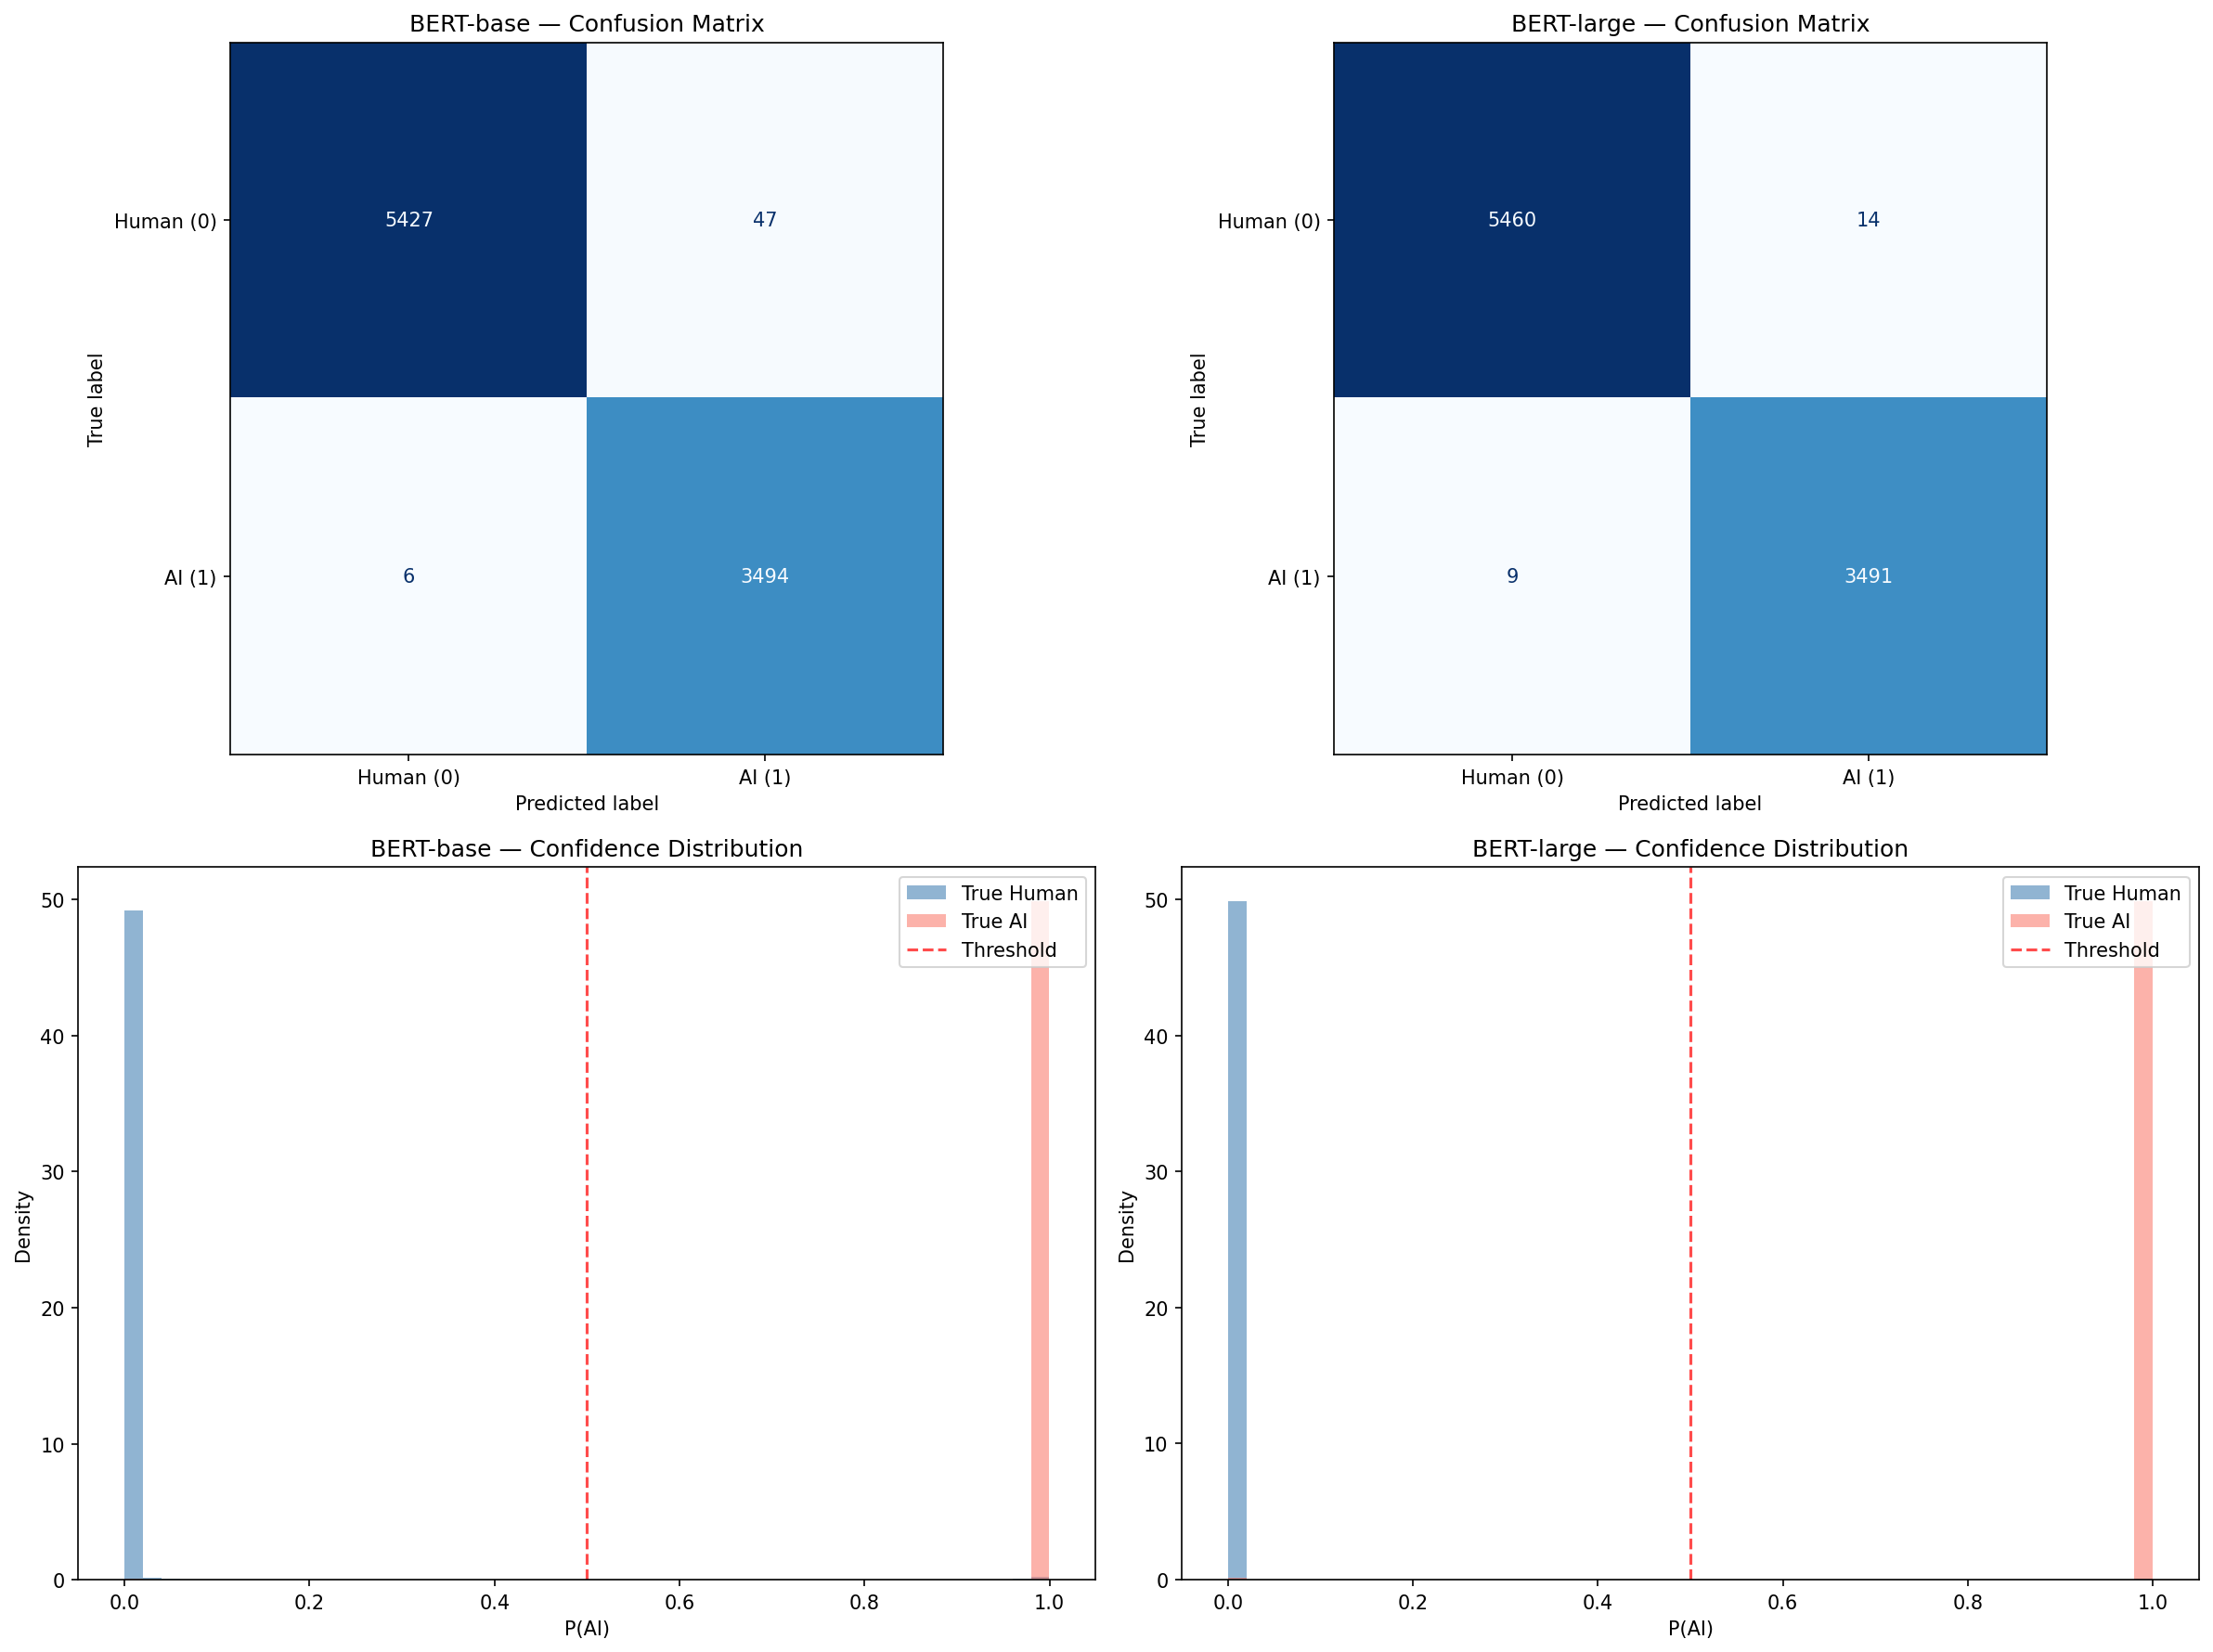
\includegraphics[width=0.85\textwidth]{results_bert-base-cased/bert_confusion_confidence.png}
\caption{Confusion matrices and confidence distributions for BERT-base and BERT-large.}
\label{fig:bert_cm}
\end{figure}

% ============================================================
\section{Adversarial Attack with Local LLM (Part 3)}
% ============================================================

\subsection{Setup}

\begin{itemize}[nosep]
\item \textbf{Local LLM}: DeepSeek-R1:8B (\texttt{deepseek-r1:8b-llama-distill-fp16}) deployed via Ollama
\item \textbf{Detector}: BERT-large-cased (3 epochs, max\_len=512)
\item \textbf{Essays}: 10 human-written essays from the validation set
\item \textbf{Strategies}: Academic rewriting, Stylistic rewriting, Paraphrase
\end{itemize}

\subsection{Single-Pass Attack Results}

\begin{table}[H]
\centering
\caption{Single-pass adversarial attack results (10 essays $\times$ 3 strategies = 30 attacks)}
\label{tab:adversarial}
\begin{tabular}{lccc}
\toprule
\textbf{Strategy} & \textbf{Attacks} & \textbf{Fooled} & \textbf{Fool Rate} \\
\midrule
Academic    & 10 & 1 & 10\% \\
Stylistic   & 10 & 0 & 0\% \\
Paraphrase  & 10 & 2 & 20\% \\
\midrule
\textbf{Total} & \textbf{30} & \textbf{3} & \textbf{10\%} \\
\bottomrule
\end{tabular}
\end{table}

\textbf{Paraphrase} is the most effective strategy (20\% fool rate) because it completely restructures vocabulary and sentence patterns, disrupting BERT's latent features.

\subsection{Iterative Attack Results}

We implemented a feedback-loop attack: after each rewrite, we report the AI probability to the LLM and ask it to further revise. Results for 5 essays with up to 3 iterations:

\begin{table}[H]
\centering
\caption{Iterative adversarial attack results (3-round feedback loop)}
\label{tab:iterative}
\begin{tabular}{lccccl}
\toprule
\textbf{Essay} & \textbf{Original} & \textbf{Iter 1} & \textbf{Iter 2} & \textbf{Iter 3} & \textbf{Fooled?} \\
\midrule
\#8927 & 0.00001 & 0.99999 & 0.99999 & 0.99999 & No \\
\#7166 & 0.00002 & 0.99999 & 0.99999 & 0.99999 & No \\
\#1744 & 0.00001 & 0.99999 & 0.99999 & 0.99999 & No \\
\#1448 & 0.00001 & 0.99999 & 0.99999 & 0.99999 & No \\
\#5258 & 0.00001 & 0.99999 & 0.99999 & 0.99999 & No \\
\bottomrule
\end{tabular}
\end{table}

\textbf{Result}: 0/5 fooled (0\%). Iterative refinement does not improve the attack success rate.

\subsection{Adversarial Examples}

\subsubsection{Example 1: Successful Attack (Essay \#1448, Paraphrase)}

\textbf{Original} (human-written, $P(\text{AI}) = 0.00001$):

\begin{quote}
``The author claim is that NASA is working on a way to visit venus despite how dangerous it is. They are planning on how they are going to visit Venus wihtout being harmed\ldots''
\end{quote}

\textbf{Rewritten} ($P(\text{AI}) = 0.2354$ --- classified as ``Human''):

\begin{quote}
``The author argues that NASA is developing a way to visit Venus despite its potential dangers. They aim to find a method to explore the planet safely, driven by the allure of discovering new things\ldots''
\end{quote}

\textbf{Why it fooled BERT}: The paraphrase smoothed grammatical errors and simplified vocabulary but preserved a student-like argumentative structure. The shortened text gave the detector less signal.

\subsubsection{Example 2: Failed Attack (Essay \#8927, All Strategies)}

\textbf{Original} ($P(\text{AI}) = 0.00001$, human):

\begin{quote}
``Having Phones at School --- Most people would like to have cell phones on there free time but some wouldn't\ldots''
\end{quote}

All three rewrites resulted in $P(\text{AI}) > 0.9999$. The LLM rewrites introduced structured paragraphs, consistent grammar, and topic sentences --- all characteristic of AI-generated text.

\begin{figure}[H]
\centering
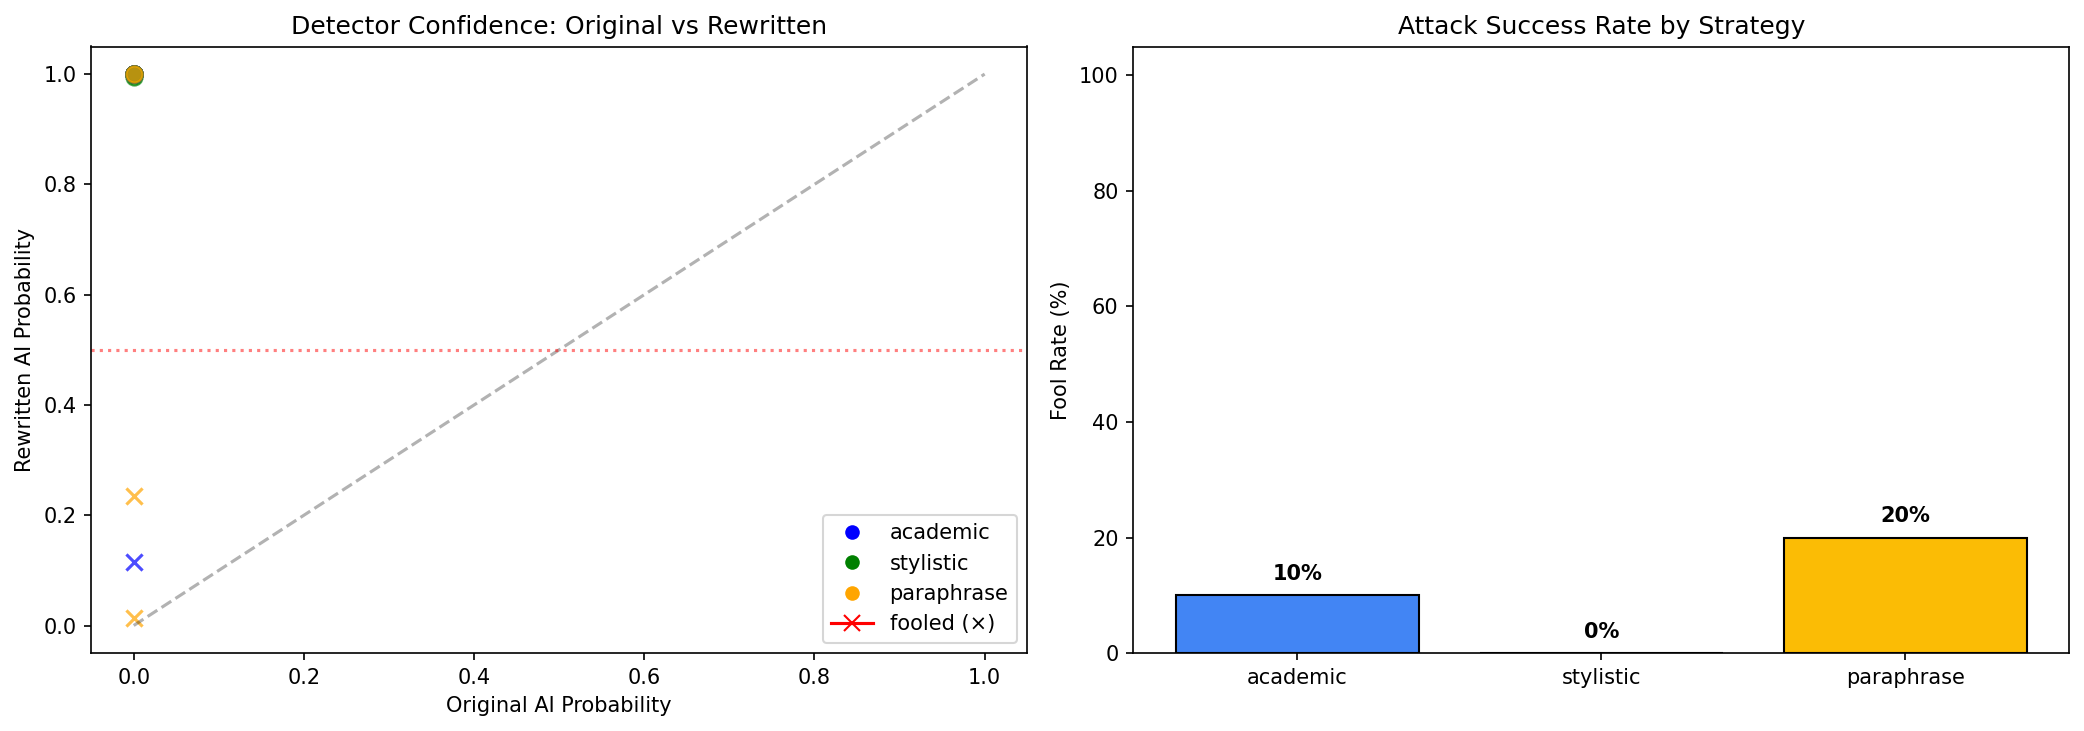
\includegraphics[width=0.85\textwidth]{results_adversarial/adversarial_attack_summary.png}
\caption{Adversarial attack summary: AI probability shift and fool rate by strategy.}
\label{fig:adversarial}
\end{figure}

\subsection{Feature Analysis of Attacks}

\begin{table}[H]
\centering
\caption{Feature changes in successful vs failed attacks}
\label{tab:feature_analysis}
\begin{tabular}{lcc}
\toprule
\textbf{Feature Change} & \textbf{Caught (avg)} & \textbf{Fooled (avg)} \\
\midrule
$\Delta$ Word Count       & $-5$   & $-30$  \\
$\Delta$ TTR              & $+0.13$ & $+0.23$ \\
$\Delta$ Avg Word Length  & $+0.2$  & $+0.3$  \\
Avg $P(\text{AI})$        & 0.9998  & 0.12   \\
\bottomrule
\end{tabular}
\end{table}

\subsection{Why BERT is Robust}

\begin{enumerate}
\item \textbf{Deep semantic understanding}: BERT captures paragraph flow, discourse structure, and vocabulary distribution patterns that survive single-pass rewrites.
\item \textbf{LLM-rewriting paradox}: Using an LLM to rewrite text \emph{replaces one AI signature with another}. In the iterative attack, human essays became \emph{more} AI-like after rewriting ($P(\text{AI})$: $\sim\!0.00001 \to \sim\!0.99999$).
\item \textbf{Training diversity}: The DAIGT V2 dataset contains AI text from multiple LLMs, making the detector generalize well across generator styles.
\item \textbf{Feature redundancy}: Both lexical features (word length, TTR) and deep features (attention patterns) point to the same classification.
\end{enumerate}

\begin{figure}[H]
\centering
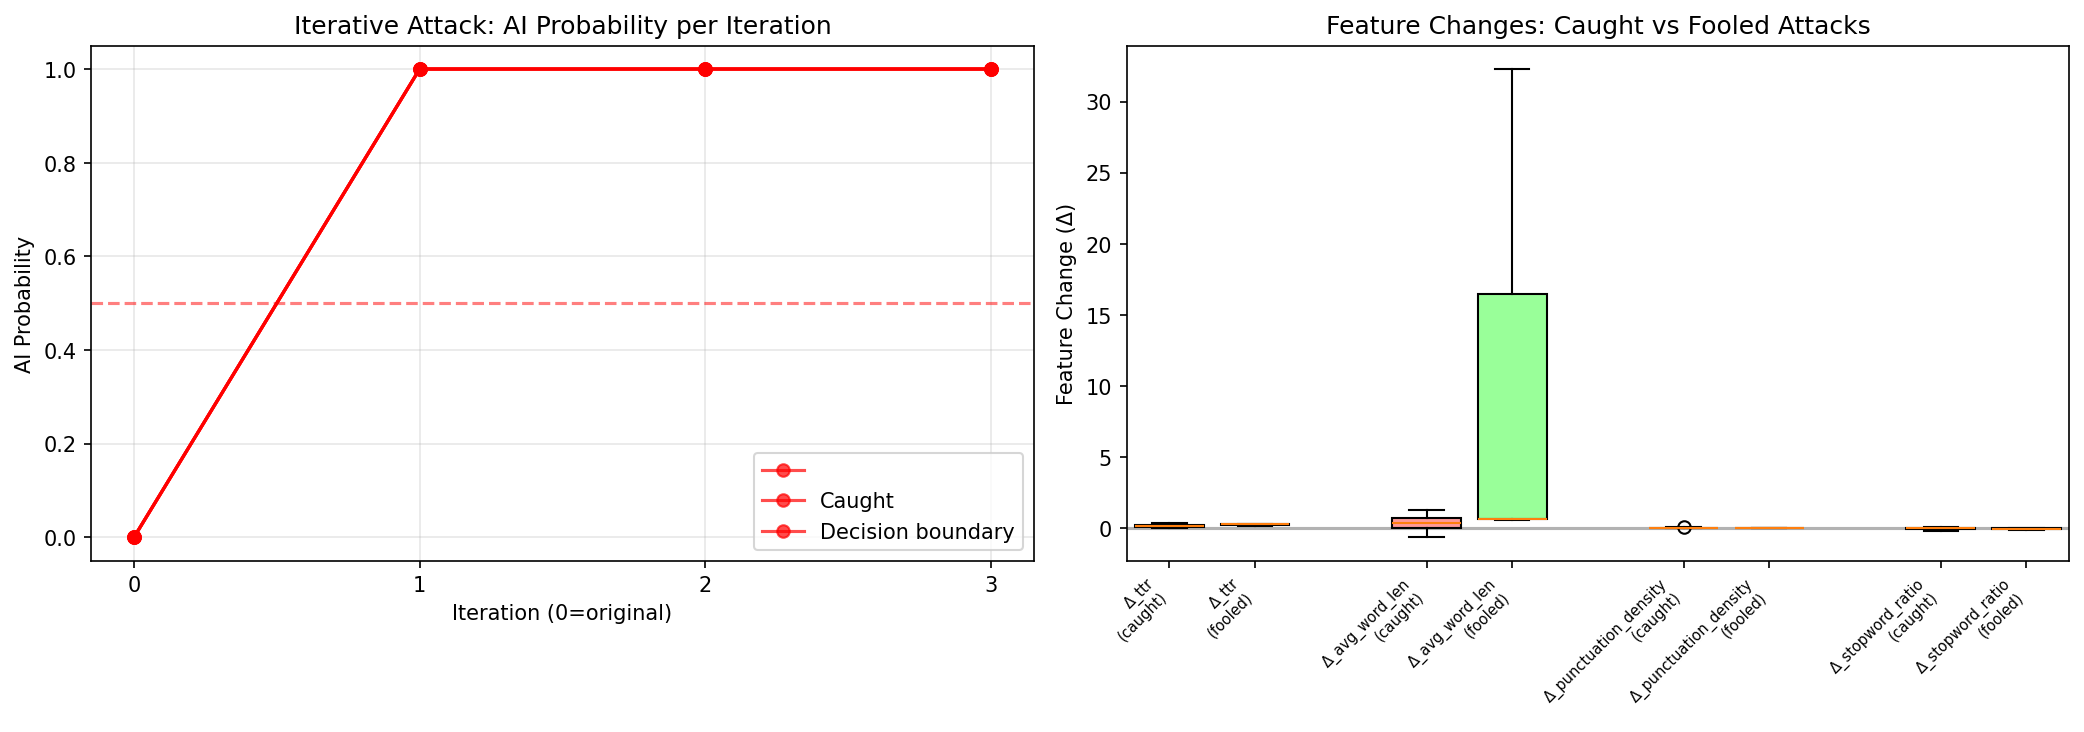
\includegraphics[width=0.85\textwidth]{results_adversarial/enhanced_adversarial_analysis.png}
\caption{Left: Iterative attack AI probability trajectory. Right: Feature change analysis (caught vs fooled).}
\label{fig:adversarial_analysis}
\end{figure}

% ============================================================
\section{Summary}
% ============================================================

\begin{table}[H]
\centering
\caption{Final performance comparison across all models}
\label{tab:summary}
\begin{tabular}{llcc}
\toprule
\textbf{Model} & \textbf{Type} & \textbf{ROC-AUC} & \textbf{Accuracy} \\
\midrule
TF-IDF + Logistic Regression & Baseline        & 0.9993 & 0.9939 \\
TF-IDF + Linear SVM          & Baseline        & 0.9997 & 0.9970 \\
BERT-base (3 epochs)          & Deep Learning   & 0.9999 & 0.9941 \\
BERT-base (5 epochs)          & Deep Learning   & 0.9999 & 0.9967 \\
BERT-large (3 epochs)         & Deep Learning   & 0.9999 & 0.9974 \\
\bottomrule
\end{tabular}
\end{table}

\textbf{Core findings}:
\begin{enumerate}
\item Both BERT models beat the TF-IDF baseline, but overall performance differences are small, reflecting task saturation.
\item BERT-large offers no meaningful ROC-AUC improvement over BERT-base despite $3\times$ the parameters and training time.
\item The BERT detector is highly robust against adversarial rewriting: only 3/30 single-pass attacks succeeded, and 0/5 iterative attacks succeeded.
\item The ``rewriting paradox'' --- LLM rewriting introduces new AI patterns --- is the fundamental reason adversarial attacks fail.
\end{enumerate}

% ============================================================
\section*{Environment}
% ============================================================

\begin{itemize}[nosep]
\item \textbf{GPU}: NVIDIA GeForce RTX 4090 (24GB VRAM)
\item \textbf{Python}: 3.13
\item \textbf{PyTorch}: with CUDA + fp16 mixed precision
\item \textbf{Transformers}: HuggingFace
\item \textbf{Local LLM}: Ollama + DeepSeek-R1:8B
\end{itemize}

\section*{Source Code}

\begin{itemize}[nosep]
\item Notebook: \texttt{HW2.ipynb}
\item Scripts: \texttt{Baseline.py}, \texttt{BERT.py}, \texttt{LocalLLM.py}
\item GitHub: \url{https://github.com/fader2077/Recurrent-Neural-Network-and-Transformer-HW/tree/main/hw2}
\end{itemize}

\end{document}
